\documentclass{article}
\usepackage{cmap}					% поиск в PDF
\usepackage[T2A, T1]{fontenc}
\usepackage[utf8]{inputenc}
\usepackage[english, russian]{babel}
\usepackage{enumitem} %[label=\alph*)]]
%%% Работа с русским языком
\usepackage{mathtext} 				% русские буквы в формулах
\usepackage{ccfonts,eulervm,euler}
\usepackage{bbding}
\usepackage{ulem}
\usepackage{indentfirst}
\usepackage{hyperref} %гиперссылки
\frenchspacing

\usepackage{fancyhdr} %Для шапки
\usepackage{amsthm}
\usepackage{amsmath}
\usepackage{amssymb} % R, Q,.
\usepackage{mathtools}
\usepackage{multicol}

\usepackage{indentfirst}
\parindent=1cm
\setlist[itemize]{itemsep=2pt, topsep=0pt} %norm lists
\setlist[enumerate]{itemsep=2pt, topsep=0pt} %norm lists

%%% Страница
\usepackage{geometry} % Простой способ задавать поля
\geometry{top=25mm}
\geometry{bottom=20mm}
\geometry{left=20mm}
\geometry{right=20mm}


%Определение, теорема, лемма, N.B.
\newtheorem*{defin*}{Определение}
\newtheorem{defin}{Определение}
\newtheorem*{Corollary*}{Следствие}
\newtheorem{Corollary}{Следствие}
\newtheorem*{Lemma*}{Лемма}
\newtheorem{Lemma}{Лемма}
\newtheorem{Theorem}{Теорема}
\newtheorem*{Theorem*}{Теорема}
\newtheorem{NB}{N.B}
\newtheorem*{NB*}{N.B}
\newtheorem{Example}{Пример}
\newtheorem*{Example*}{Пример}

%Proof
\newenvironment{Proof}
{\par\noindent{\bf Доказательство.}} 
{\hfill$\scriptstyle\blacksquare$}

\newcommand{\eq}[1][m]{\mathop{\equiv}\limits_{#1}}

\newcommand{\smallheader}[1]{\noindent{\bf #1 }}

\newcommand{\divs}{\,\lower.4ex\vdots\,}% a делится на b

\newcommand{\rmy}[1][m]{\mathbb{R}^{#1}}%$R^m$

\newcommand{\eqdef}{\overset{def}{\underset{}{=}}}% =def

\newcommand{\shapka}[1]{\pagestyle{fancy}\fancyhead[C]{#1}\fancyfoot{}}%Шапка

\newcommand{\chast}[2]{\dfrac{\partial #1}{\partial #2}}

%TADA https://youtu.be/9Cq56iPTQ5A?t=20
\newcommand{\THEN}{\text{\href{https://youtu.be/9Cq56iPTQ5A?t=20}{Тогда }}}

\usepackage{listings}
\usepackage{xcolor}

%New colors defined below
\definecolor{codegreen}{rgb}{0,0.6,0}
\definecolor{codegray}{rgb}{0.5,0.5,0.5}
\definecolor{codepurple}{rgb}{0.58,0,0.82}
\definecolor{backcolour}{rgb}{0.95,0.95,0.92}

%Code listing style named "mystyle"
\lstdefinestyle{mystyle}{
	backgroundcolor=\color{backcolour},   commentstyle=\color{codegreen},
	keywordstyle=\color{magenta},
	numberstyle=\tiny\color{codegray},
	stringstyle=\color{codepurple},
	basicstyle=\ttfamily\footnotesize,
	breakatwhitespace=false,         
	breaklines=true,                 
	captionpos=b,                    
	keepspaces=true,                 
	numbers=left,                    
	numbersep=5pt,                  
	showspaces=false,                
	showstringspaces=false,
	showtabs=false,                  
	tabsize=2
}

\lstset{style=mystyle}

\title{Code Listing}


\begin{document}
	\shapka{Клепов Дмитрий (M3238)\\
		Обратная связь: dimkakirov43@mail.ru}
	{\bf Вариант 9}
	
	\textbf{Задание}.
	
	Для заданной квадратичной функции $y = a_3+a_2 x+a_1 x^2$
	\begin{itemize}
		\item Смоделировать квадратичную функцию, наблюдаемую в нормальных шумах
		\item Оценить коэффициенты квадратичной зависимости, уровень шумов и квадратичную функцию по зашумленным данным
		\item Сравнить полученные результаты с исходными данными.
		\item Проделать аналогичное с прямой $y=c_2+c_1 x$
	\end{itemize}

	\textbf{Исходные данные}
	\begin{itemize}
		\item $x_{min}=-0.5$
		\item $x_{max}=1.5$
		\item $n=50$
		\item $y=3.5-2.2x+1.2x^2$, $y=2.8+1.3 x$
		\item $s=2.3$
	\end{itemize}
	
	\bigskip
	
	{\bf Графики.}\\
	
	\begin{figure}[h]
		\centering
		\begin{minipage}{0.45\textwidth}
			\centering
			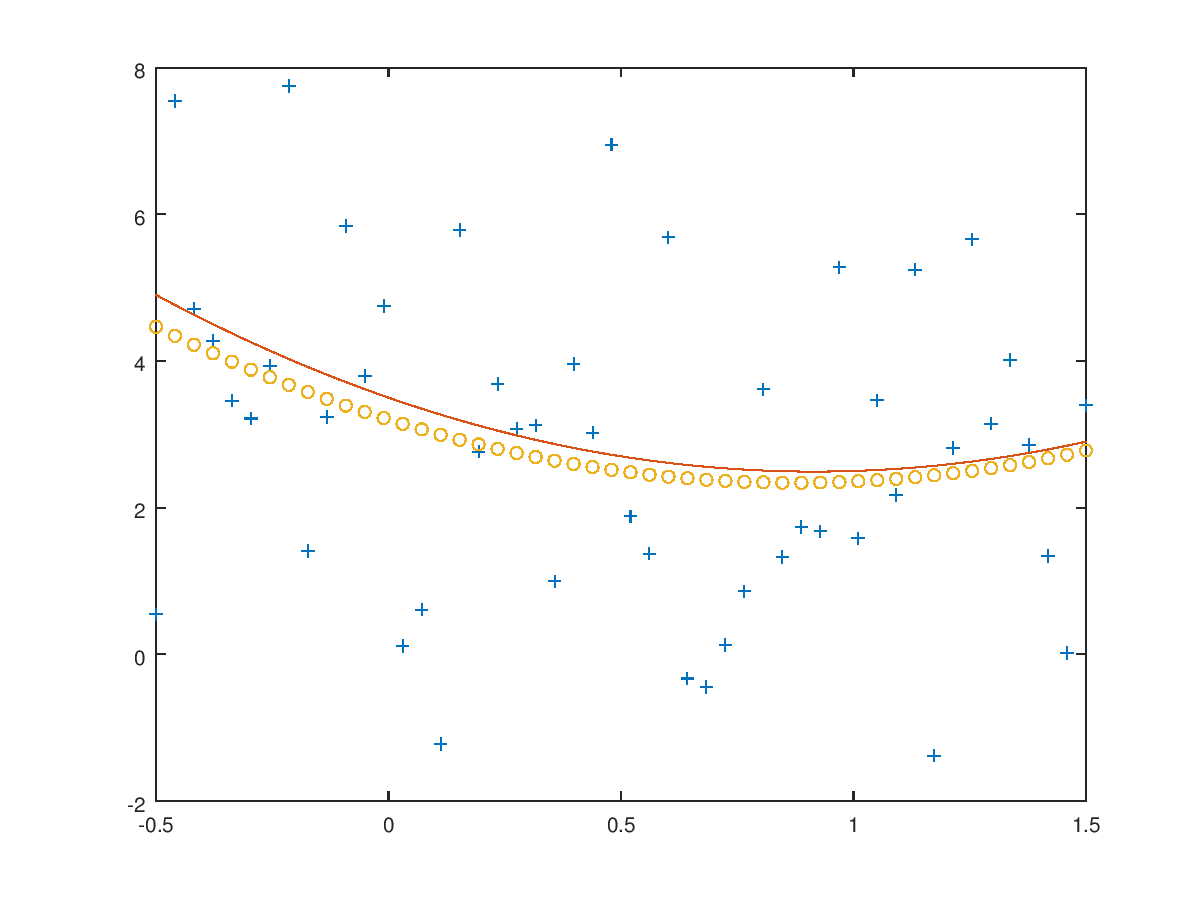
\includegraphics[width=\textwidth]{quad.png}
			\caption{Квадратичная}
		\end{minipage}\hfill
		\begin{minipage}{0.45\textwidth}
			\centering
			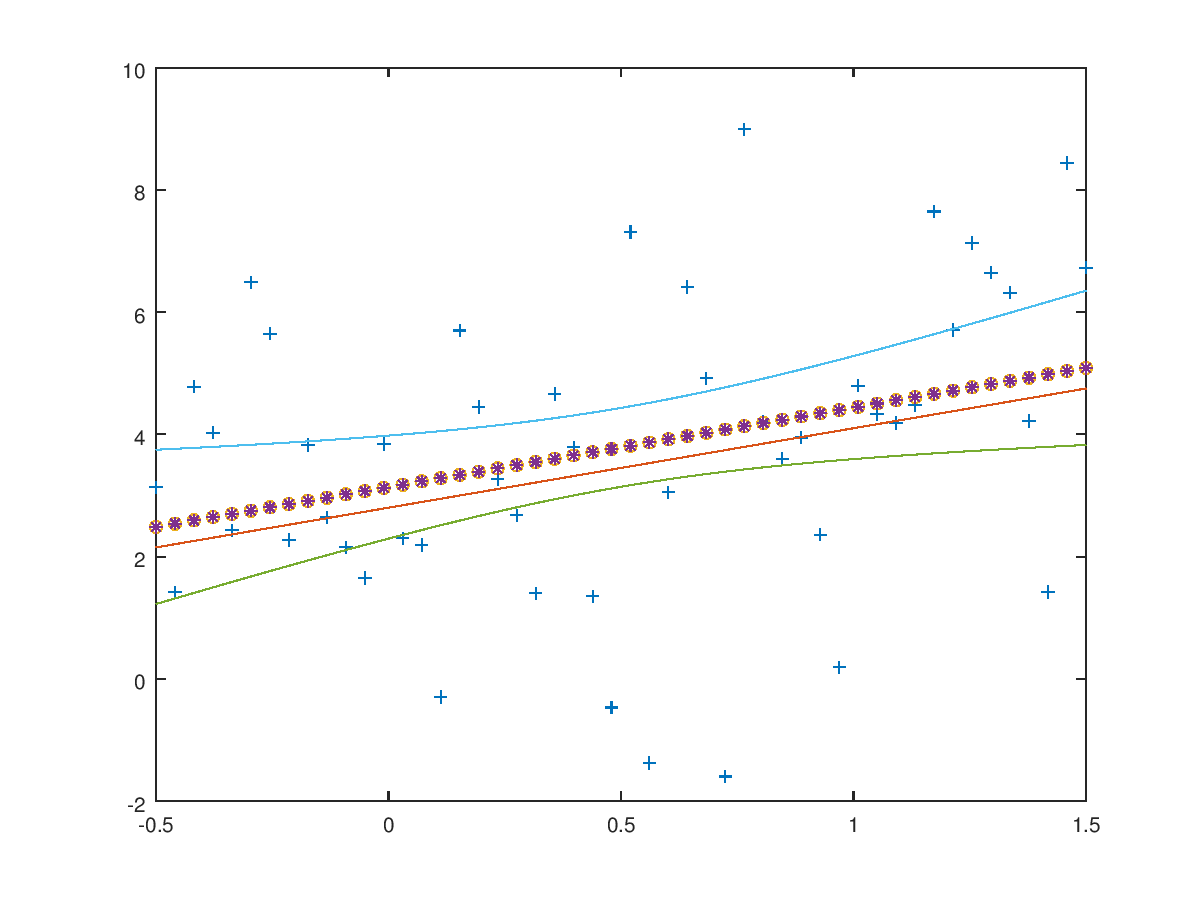
\includegraphics[width=\textwidth]{linear.png}
			\caption{Линейная}
		\end{minipage}
	\end{figure}

	\begin{itemize}
		\item Квадратичная:
		\lstinputlisting[language=Octave]{quad.m}
		
		{\bf Выход:}\\
		\begin{lstlisting}
		Noise: 2.473507
		Ort check: -0.000000\end{lstlisting}
		
		
	
		\item Линейная:
		\lstinputlisting[language=Octave]{linear.m}
		
		{\bf Выход:}\\
		\begin{lstlisting}
		Diff: 1.369099
		Ort check: -0.000000
		Noise: 2.617631\end{lstlisting}
		
	\end{itemize}
	
	\textbf{Вывод:} (для обеих)
	\begin{itemize}
		\item Полученная функция почти совпадает с исходной
		\item Полученный уровень шумов близок к заданному
		\item Вектор несвязок ортогонален вектору зашумленной функции
	\end{itemize}
	Для линейной: функция попала в доверительный интервал.
	
\end{document}
